\documentclass[12pt, a4paper]{book}
%% Packages élémentaires %%
\usepackage[utf8]{inputenc}
\usepackage{mathpazo,etoolbox, graphicx, wrapfig, pbox, fancybox, hyperref, appendix, geometry, amsmath, amssymb, tikz, pgfplots, calc, enumitem, colortbl
}
\newcommand{\cst}{\text{c}^{\text{\scriptsize ste}}}
\newcommand{\ddx}{\dfrac{\textrm d ^2 x}{\textrm d t^2}}
\renewcommand{\d}{\mathrm{d}}
\newcommand{\dx}{\mathrm{d}x}
\newcommand{\dy}{\mathrm{d}y}
\newcommand{\dz}{\mathrm{d}z}
\newcommand{\dt}{\mathrm{d}t}
\newcommand{\dxp}{\mathrm{d}x'}
\newcommand{\dyp}{\mathrm{d}y'}
\newcommand{\dzp}{\mathrm{d}z'}
\newcommand{\dtp}{\mathrm{d}t'}
\newcommand{\dvx}{\mathrm{d}\vec x}
\newcommand{\dvxp}{\mathrm{d}\vec x'}
\newcommand{\ch}{\mathrm{ch}}
\newcommand{\sh}{\mathrm{sh}}
\renewcommand{\th}{\mathrm{th}}
\newcommand{\tg}{\mathrm{tg}}
\newcommand{\C}{\textbf{C} }
\newcommand{\Cpp}{\textbf{C}++ }
\newcommand{\ud}[3]{{#1}^{#2} _{\; {#3} }}
\newcommand{\du}[3]{{#1}_{#2} ^{\; {#3} }}
\newcommand{\dd}[3]{{#1}_{#2} _{\; {#3} }}
\newcommand{\uu}[3]{{#1}^{#2} ^{\; {#3} }}
\setlength{\parindent}{0pt}

\graphicspath{{images/}}
\geometry{hmargin=2.4cm, vmargin = 2.1cm}
\setlist[itemize]{itemsep=10pt, label={--}}

%% Couleurs %%
\usepackage{xcolor}
\definecolor{bleu}{RGB}{14, 68, 175}
\definecolor{BGbleu}{RGB}{222, 233, 255 }
\definecolor{BGorange}{RGB}{255, 216, 154}
\definecolor{rouge}{RGB}{201, 0, 0}
\definecolor{vert}{RGB}{14, 137, 0}
\definecolor{BGgris}{RGB}{222,230,230}
\newcommand\rouge[1] {{\color{rouge}{#1}}}
\newcommand\bleu[1] {{\color{bleu}{#1}}}
\newcommand\green[1]{{\color{vert}{#1}}}


%% Cadres %%
\newcommand\bbm[1]{
\begin{center}
\fcolorbox{black}{BGbleu}{\parbox{\linewidth}{ 
#1
}}
\end{center}}
\newcommand\bo[1]{
\begin{center}
\fcolorbox{black}{BGorange}{\parbox{\textwidth}{ 
#1
}}
\end{center}}

\newcommand\bb[1]{
\begin{center}
\fcolorbox{black}{BGbleu}{\parbox{\textwidth}{ 
\begin{Large}
\begin{center}
#1
\end{center}
\end{Large}
}}
\end{center}}
\renewcommand\bo[1]{
\begin{center}
\fcolorbox{black}{BGorange}{\parbox{\textwidth}{ 
#1
}}
\end{center}}

\newcommand\boite[1]{
\begin{center}
\fbox{\parbox{\textwidth}{#1}}
\end{center}}



\newcommand\aparte[1]{
\begin{center}
\fcolorbox{white}{BGgris}{\parbox{\linewidth}{ \textit{A parte} \\
#1 }}
\end{center}}
\newcommand\bg[2]{
\begin{center}
\fcolorbox{white}{BGgris}{\parbox{\linewidth}{\begin{large} \textit{#1} \end{large} \\

#2 }}
\end{center}}

\newcommand\exemple[1]{
\begin{center}
\fcolorbox{white}{BGgris}{\parbox{\linewidth}{ \textit{Exemple} \\
#1 }}
\end{center}}

%% Commandes %%
\newcommand\imp[1]{\underline{\textbf{#1}}}
\newcommand\eq[1]{\begin{large}
\begin{align*}
#1
\end{align*}
\end{large}}
%% Commandes fantaisistes (cf. Internet) %%
\renewcommand{\parallel}{ \mathbin{\!/\mkern-5mu/\!} }
\newcommand{\q}[1]{{%
\font\larm = larm1000%
\larm%
\char 190}{ \textit{#1} }{%
\font\larm = larm1000%
\larm%
\char 191}}

%% Wrapping %%
\newcommand\wrap[4]{\begin{wrapfigure}[#1]{#2}{#3\textwidth}
#4
\end{wrapfigure}}
%% TikZ
\usepackage{pgfplots}
\usetikzlibrary{shapes}
\usetikzlibrary{calc}
\usetikzlibrary{positioning}
\usetikzlibrary{intersections}
\usetikzlibrary{angles}
\usetikzlibrary{quotes}
\newcommand{\drawaxes}[3]{
\coordinate (o) at #1 ;
\draw[->] ($(o) + (-0.1*#2, 0)$) --+ (#2, 0) ;
\draw[->] ($(o) + (0,-0.1*#3)$) --+ (0,#3) ;
}

\newcommand{\drawthickaxes}[5]{
\coordinate (o) at #1 ;
\draw[thick,->] ($(o) + (-0.1*#2, 0)$) --+ (#2, 0) node[anchor = north east]{#4};
\draw[thick,->] ($(o) + (0,-0.1*#3)$) --+ (0,#3) node[anchor = north east]{#5};
}

\newcommand*{\ShowIntersectionWithSinAbs}{
\fill 
    [name intersections={of=DroiteK and SinAbs, name=i, total=\t}] 
    [red, opacity=1, every node/.style={above left, black, opacity=1}] 
    \foreach \s in {1,...,\t}{
        \ifodd \s 
        {}
        \else
        (i-\s) circle (2pt) node [above] {\s} 
        \fi 
        };
}
\newcommand*{\ShowIntersectionWithCosAbs}{
\fill 
    [name intersections={of=DroiteK and CosAbs, name=i, total=\t}] 
    [blue, opacity=1, every node/.style={above left, black, opacity=1}] 
    \foreach \s in {1,...,\t}{
        \ifodd \s 
        (i-\s) circle (2pt) node [above] {\s} 
        \fi 
        };
}

%% Code %%
\usepackage{listings}
\definecolor{codegreen}{rgb}{0,0.6,0}
\definecolor{codegray}{rgb}{0.5,0.5,0.5}
\definecolor{codepurple}{rgb}{0.58,0,0.82}
\definecolor{backcolour}{RGB}{242,242,242}
\definecolor{codeorange}{RGB}{255,140,0}
% https://gist.github.com/nhtranngoc/88b72d9bfb656a3de227eea38ed80627
\definecolor{background}{RGB}{39, 40, 34}
\definecolor{string}{RGB}{230, 219, 116}
\definecolor{comment}{RGB}{117, 113, 94}
\definecolor{normal}{RGB}{248, 248, 242}
\definecolor{identifier}{RGB}{166, 226, 46}

\newcommand{\code}[1]{\texttt{{\color{codepurple}{#1}}}}
\newcommand{\codep}[1]{\texttt{{\color{codegreen}{#1}}}}

\lstdefinestyle{mystyle}{
    backgroundcolor=\color{backcolour},   
    commentstyle=\color{bleu},
    keywordstyle=\color{codeorange},
    numberstyle=\tiny\color{codegray},
    stringstyle=\color{codepurple},
    basicstyle=\ttfamily\footnotesize,
    breakatwhitespace=false,         
    breaklines=true,                 
    captionpos=b,                    
    keepspaces=true,                 
    numbers=left,                    
    numbersep=5pt,                  
    showspaces=false,                
    showstringspaces=false,
    showtabs=false,                  
    tabsize=2
}

\lstdefinestyle{py}{
	language=python,
    backgroundcolor=\color{backcolour},   
    commentstyle=\color{bleu},
    keywordstyle=\color{codeorange},
    numberstyle=\tiny\color{codegray},
    stringstyle=\color{codepurple},
    basicstyle=\ttfamily\footnotesize,
    breakatwhitespace=false,         
    breaklines=true,                 
    captionpos=b,                    
    keepspaces=true,                 
    numbers=left,                    
    numbersep=5pt,                  
    showspaces=false,                
    showstringspaces=false,
    showtabs=false,                  
    tabsize=2
}

\lstset{style=mystyle}
\lstset{language=C}

\lstdefinestyle{cppstyle}{
basicstyle=\footnotesize\sffamily\color{black},
commentstyle=\color{mygray},
frame=single,
numbers=left,
numbersep=5pt,
numberstyle=\tiny\color{mygray},
keywordstyle=\color{mygreen},
showspaces=false,
showstringspaces=false,
stringstyle=\color{myorange},
tabsize=2
}

\usepackage{framed}

\renewenvironment{leftbar}[1][\hsize]
{%
     \def\FrameCommand
     {%
         {\color{black}\vrule width 3pt}%
         \hspace{7pt}%must no space.
        % \fboxsep=\FrameSep\colorbox{yellow}%
     }%
     \MakeFramed{\hsize#1\advance\hsize-\width\FrameRestore}%
}
{\endMakeFramed}

\usepackage[french]{babel}
\usepackage{titling, setspace, anyfontsize, amsthm}
\newcommand\psirt{\psi(\vec{r},t)}
\newcommand\psikrt{\psi_{\vec{k}}(\vec{r},t)}
\newcommand\drawline[1]{%
     \begin{tikzpicture}                                                           
       \draw[#1] (0pt,0pt) -- (15pt,0pt);                                       
     \end{tikzpicture}%
} 

\newcommand\documentname[4]{\title{
	
\includegraphics[width=0.4\textwidth]{Logo-Sciences-ULB} \\
	\vspace{2cm}
    \includegraphics[width=1\textwidth]{#3} \\
    \includegraphics[width=1\textwidth]{#4} \\
    \vspace{0.7cm}
     #1\\
    \vspace{0.6cm}
    \LARGE ULB -- Faculté des Sciences\\ 
    \vspace{0.7cm}
    \large #2
    \vspace{0.8cm}
}}

\documentname{Introduction à la mécanique quantique}{B2-PHYS : PHYS-F203 -- Pr. \textsc{Massar}}{pqs-cover_1}{pqs-cover_2}
\author{Sami \textsc{Abdul Sater}}
\date{\hspace{-0cm}Année académique 2020-2021}

\begin{document}

\maketitle
\vfill


\thispagestyle{empty}
\restoregeometry
\tableofcontents
\chapter{Principes fondamentaux de la physique quantique}

\section{Dualité onde-corpuscule de la lumière}
La lumière a toujours été dans l'histoire une source d'interrogation. Elle nous sert à voir littéralement, mais certaines manipulations avec permettent d'en étudier la nature. Corpuscule ? Ondulatoire ? Les deux hypothèses se combattaient au XVIIè siècle, avec Christophe Huygens qui défendait une théorie ondulatoire et Isaac Newton qui défendait une théorie corpusculaire. \\

Au XIXè siècle, des expériences de diffraction (phénomène purement ondulatoire) menées par Thomas Young et Augustin Fresnel ont permis d'affirmer que la lumière possédait des propriétés ondulatoires. Newton part donc avec un point en moins. Un siècle plus tard, Einstein émet une théorie corpusculaire de la lumière, certaines raisons l'ayant poussé à le faire. Parmi eux, les travaux de Planck. \\

Max \textsc{Planck} étudiait les corps noirs (enceinte macroscopique à l'équilibre thermodynamique) et de ses études est ressorti un paramètre qui a les dimensions $\mathrm{E} \times \mathrm{T} \equiv \mathrm{Js}$ ou \textit{action}. Ce paramètre qu'on note $h$ décrit formidablement les propriétés des corps noirs. L'étude de Max Planck aboutissait à une conclusion que l'énergie d'un corps noir est quantifiée. De l'autre côté, Einstein décrit également \textbf{l'effet photoélectrique} \footnote{Effet expliquant l'émission d'électrons par un métal exposé à de la lumière dans certaines conditions.} avec cette constante. Ceci souligne l'importance de $h$ car le corps noir et le métal n'ont \textit{a priori} rien en commun. La constante de Planck est donc une des \textit{constantes de l'Univers}.
$$h \approx 6.63 ; 10^{-34} \; \mathrm{Js}$$

\subsubsection{Effet photoélectrique}
En bombardant une plaque métallique de lumière de longueur d'onde $\lambda$ (maintenant qu'on sait que la lumière est une onde), on remarque qu'au-delà d'une certaine fréquence $\nu_0$ ($\lambda$ et $\nu$ sont liées par $\lambda = c/\nu$), des électrons sont émis avec une énergie qui augmente linéairement avec la fréquence, avec une pente de $h$.

$$ T = h\nu - W \qquad \text{où} \quad W = h\nu_0 $$
$W$ est le travail que fournit la lumière, l'énergie associée à un rayonnement de fréquence $\nu_0$.

\subsubsection{Les particules de lumière}
Einstein est amené à établir une relation entre la longueur d'onde de la lumière et une impulsion (à travers le nombre d'onde, ou plus précisément, le vecteur d'onde $\vec{k}$). Ce faisant, il donne aux quantas d'énergie toutes les propriétés d'une particule. Comme l'énergie et liée à la pulsation $\omega$ et l'impulsion est lié au vecteur d'onde $\vec{k}$, on peut lier le quadrivecteur $\mathrm{P}$ à un autre quadrivecteur, le \q{quadrivecteur d'onde} $\mathrm{K}$.
\begin{center}
$\left\{ \begin{array}{l}
E \equiv \hbar \omega \quad \text{\small (quantification de l'énergie}) \\
\vec{p} \equiv \hbar \vec{k}  \quad \text{\small (lien longueur d'onde-impulsion)}
\end{array} \right.
\quad \Longrightarrow \quad 
\left\{ \begin{array}{l}
\mathrm{P} \equiv (E/c, \vec{p}) \\
\mathrm{K} \equiv (\omega/c, \vec{k})
\end{array} \right. \quad \Rightarrow \quad \boxed{\mathrm{P} = \hbar \mathrm{K}}$
\end{center}
Pour une particule de lumière, la relation de dispersion, c'est-à-dire le lien entre la pulsation et le nombre d'onde, est donnée par  $\omega = kc$. Ceci implique par la quantification de l'énergie $E = pc$, ce qui est la caractéristique d'une particule de masse nulle. La lumière est ainsi faite de particules de masse nulle. \\

L'introduction d'une particule de lumière, a.k.a le \textbf{photon} n'est pas super appréciée et nécessite donc d'être démontrée. C'est ce qu'a fait Arthur Compton expérimentalement. Il a démontré que lors d'une interaction (une collision) photon-électron, l'impulsion et l'énergie du photon étaient conservées, tout comme une particule classique. Le photon est donc bien une particule. Eeeet c'est aussi une onde (\textit{cf.} franges de Young). 
\begin{center}
\begin{large}
\textit{La lumière est donc une onde \underline{et} faite de particules.}
\end{large}
\end{center}

\subsection{Observation de la dualité onde-particule de la lumière}
On reprend l'expérience des fentes de Young et cette fois-ci en lumière atténuée, pour voir la figure d'interférence se construire progressivement. On alors les impacts un par un, \textbf{photon par photon} mais à long terme on voit se dessiner une figure d'interférence, cela veut dire que la lumière est une onde qui passe par les deux fentes à la fois.

\begin{itemize}
\item Nature corpusculaire : les impacts individuels.
\item Nature ondulatoire : la lumière passe par les deux fentes à la fois (figure d'interférence).
\item Dualité onde-particule : la lumière est à la fois partout et à un seul endroit. \end{itemize}

Une grande morale à cette section est que mine de rien, Einstein a développé et cru en une théorie qui allait à l'encontre de ce qui a été imaginé et prouvé par l'expérience depuis le siècle le précédant, et ce malgré la splendide explication théorie de l'électromagnétisme de Maxwell. Aucune invalidité dans un modèle prouvé par l'expérience ! Mais il y avait visiblement de la place pour une autre théorie. 
\section{Dualité onde-corpuscule de la matière}
L'aspect corpusculaire de la matière n'a pas besoin d'être introduit. En revanche, son aspect ondulatoire nourrit les interrogations rien qu'à l'usage de l'expression. C'est Louis de Broglie le véritable héros derrière cette hypothèse.
\subsection{Hypothèse de De Broglie}
L'aspect corpuscule de la lumière a été observé lors de l'effet Compton. L'effet photoélectrique permet de donner un lien entre les nature corpuscule et ondulatoire de la lumière : un rayonnement de fréquence $\nu$ est porteur d'une énergie $E = h\nu$. Une autre relation peut être déduite par calcul pour obtenir l'impulsion correspondant à ce photon. Ce sont les relations onde-corpuscule de la lumière :
\begin{equation}
\boxed{
\text{Relation onde-corpuscule (photon) : } \quad \left\{ \begin{array}{ll}
E &= h\nu \\
\vec p &= \frac{h}{2\pi} \vec k
\end{array} \right. } \; .
\end{equation}

À cette époque, on étudie les spectres d'émission et d'absorption de certains atomes, où on les voit constitués de raies fines : un atome émet et absorbe des photons d'énergies bien déterminées. En passant d'un état à un autre, un photon d'énergie $E_{ij}$ est produit, où
$$E_{ij} = h\nu_{ij} = |E_i - E_j| \; .$$
Cet effet a d'ailleurs été confirmé par Franck et Hertz. \\

\wrap{15}{r}{0.4}{\centering \vspace{-0.5cm}
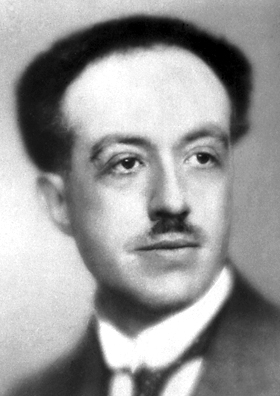
\includegraphics[width=0.6\linewidth]{Louis_de_Broglie}
\caption{Louis de Broglie. Il obtint le prix Nobel en 1929 à 37 ans pour la découverte de la nature ondulatoire de l'électron.}}

Louis de Broglie émet alors l'hypothèse que \textbf{tous les corpuscules matériels peuvent avoir un aspect ondulatoire}, et que les aspects corpuscule et ondulatoire sont reliés par la formule \eqref{eq:debroglie}.
\begin{equation} \label{eq:debroglie}
\boxed{
\text{Relations de De Broglie : } \quad \left\{ \begin{array}{ll}
E &= \hbar \omega \\
\vec p &= \hbar \vec k
\end{array} \right. } 
\end{equation}

Il faut bien comprendre l'étape à laquelle nous sommes de la construction d'une nouvelle physique. En tout premier lieu, \textbf{quelque chose n'allait pas} dans le modèle actuel et c'était les propriétés ondulatoire et corupusculaire de la lumière : les deux étaient prouvés expérimentalement. En introduisant la dualité onde-corpuscule, ce problème disparaissait et tous les résultats tenaient. Ce concept a été formulé par De Broglie pour les particules de matières telles que l'électron et a fini par être également vérifié. De Broglie généralise les relations d'Einstein pour le photon et nous avons donc à notre disposition des \textit{relations} pour décrire les particules au niveau microscopique (\ref{eq:debroglie}). \\

Pour obtenir une \textit{physique}, il faut encore (au moins) avoir une équation qui décrit le comportement d'une particule. Une particule est également une onde. Ce qui peut alors être fait est de décrire une particule par une équation d'onde (l'équation d'onde EM pour le photon), et d'obtenir son énergie et son impulsion par les relations de De Broglie. Mais pour se faire, il faut avoir à disposition une équation d'onde. L'équation qui décrit une particule quantique (et plus tard, son évolution) est l'équation de Schrödinger. La section qui suit montre comment \textbf{construire} une fonction d'onde à partir d'analogies mathématiques avec la fonction d'onde EM et à partir des relations que nous venons d'obtenir (\ref{eq:debroglie}).

\subsection{Vers l'équation de Schrödinger}
Tout comme pour l'équation d'onde du photon, établissons une équation d'onde dont la solution sera la fonction d'onde d'un corpuscule matériel. La première étape sera d'\textbf{établir une équivalence} entre des grandeurs physiques et des opérateurs. Ensuite, il suffira de relier les grandeurs physiques entre elles et on obtiendra une équation liant plusieurs aspects de la fonction d'onde (mélange d'opérateurs).\\

\begin{enumerate}[label =  (\alph*)]
\item \textit{Équivalence entre opérateurs}. \\
L'équation d'onde du photon est
$$\left(\dfrac{1}{c^2} \partial_t ^2 - \Delta \right) \vec A = 0$$
et sa solution est $$
A = A_0 \; e^{-i(\omega t - \vec k \cdot \vec x)} \; .$$
De ce fait, nous pouvons déduire que 
\begin{itemize}
\item dériver $A$ par rapport au temps devient à multiplier $A$ par $-i\omega$,
$$\boxed{\omega \longleftrightarrow \dfrac{i}{A} \partial_t A} \; , $$
\item prendre le gradient revient à multiplier par $i\vec k$, 
$$\vec k \longleftrightarrow -\dfrac{i}{A} \vec \nabla A \quad \Rightarrow \quad \boxed{k^2 \longleftrightarrow -\dfrac{1}{A} \Delta A} \; .$$
\end{itemize}

\item \textit{Recherche d'une relation à exploiter}. \\
Dans le cas d'un photon, l'équation d'onde était directement obtenue par les équations de Maxwell, la résolution était simple et on a pu en déduire une équivalence entre opérateurs. Dans le cas d'un corpuscule matériel, on souhaite partir d'une équivalence pour construire une équation qu'on espère pouvoir résoudre. Avec la règle de correspondance pour la pulsation et le vecteur d'onde de l'équivalent ondulatoire de notre corpuscule, nous pouvons, pour construire une équation d'onde, l'appliquer à une équation qui lie $\omega$ et $\vec k$, ou une équation qui lie $E$ et $\vec p$, leur étant respectivement proportionnels. Or c'est exactement ce que nous fournit i) la norme du quadri-vecteur énergie-impulsion de la particule dans le cas relativiste, et ii) la conservation de l'énergie dans le cas classique. Écrivons la règle de correspondance pour une particule quantique pour ensuite écrire les relations entre $E$ et $\vec p$ pour construire une équation d'onde.

\begin{equation} \label{eq:ch2-correspondance}
\left\{ \begin{array}{lll}
E &= \hbar \omega &= \dfrac{i\hbar}{\psi} \partial_t \psi \\
\vec p &= \hbar \vec k &= -\dfrac{i\hbar}{\psi} \vec \nabla \psi \Rightarrow p^2 = -\dfrac{\hbar ^2}{\psi} \Delta \psi
\end{array} \right. \Longrightarrow \quad \boxed{\begin{array}{ll}
E &=\dfrac{i\hbar}{\psi} \partial_t \psi \\
p^2 &=  \dfrac{i\hbar}{\psi} \partial_t \psi
\end{array}}
\end{equation}

\begin{enumerate}[label = \roman*)]
\item Cas relativiste : 
$$E^2 = m^2 c^4 + p^2 c^2$$
La substitution des relations de \eqref{eq:ch2-correspondance} dans cette relation décrit le comportement d'une particule quantique relativiste et constitue l'\textbf{équation de Klein-Gordon}.
\begin{equation} \label{eq:dirac}
\boxed{\text{Équation de Klein-Gordon} : \quad -\hbar ^2 \partial_t ^2 \phi + c^2 \hbar ^2 \Delta \phi - c^4 m^2 \phi = 0}
\end{equation}
Cette équation sera traitée en BA3. De ce que l'on peut voir, elle est d'ordre 2 en le temps ce qui est le signe de fréquences positive et négative, et [...]
\item Cas non-relativiste :
$$E = \dfrac{p^2}{2m} + V(\vec r, t)$$
De manière similaire, on obtient l'équation de \textbf{Schrödinger} :
\begin{equation} 
\boxed{\text{Équation de Schrödinger} : \quad
i\hbar \dfrac{\partial}{\partial t} \psi = -\dfrac{\hbar ^2}{2m} \Delta \psi + V(\vec r, t) \psi}
\end{equation}

\end{enumerate}
\end{enumerate}
Nous voyons donc qu'en suivant ces deux procédures, nous pouvons arriver à trouver une expression décrivant la physique d'une particule dans certaines situations. Le cas non-relativiste d'une particule est celui que nous allons étudier profondément cette année. C'est d'ailleurs le sujet de tout le chapitre suivant, où ses propriétés et son interprétation sont discutées, et quelques exemples sont traités.

\chapter{L'équation de Schrödinger}
Les résultats du chapitre précédent ont permis de mettre en évidence certaines observations qui ont fini par constituer les principes fondamentaux de la physique quantique. Son résultat notable a été l'obtention d'une équation qui régit le comportement d'une particule quantique, à la fois celui d'une onde et d'un corpuscule. Dans le régime non-relativiste, cette équation s'appelle \textbf{équation de Schrödinger}. Dans ce chapitre, nous expliciterons son intérêt mathématique, son contenu physique (interprétation), et enfin traiterons quelques exemples de résolution avec différents cas de potentiels. Nous verrons en effet qu'une simple étude de cette équation mène a des résultats qui diffèrent radicalement de la physique classique et qui ont un intérêt non-négligeable, comme l'effet tunnel. 

\bb{Équation de Schrödinger 
\begin{equation}\label{eq:schrodinger}
  i\hbar\;  \dfrac{\partial}{\partial t}\;  \psi \quad = \quad  -\dfrac{\hbar ^2}{2m} \; \Delta \psi + V(\vec r, t) \;  \psi
\end{equation}
}

\section{Étude mathématique}
Dans cette section nous verrons plusieurs choses :
\begin{table}[h!]
  \centering
  \begin{tabular}{r|p{10cm}}
    Résolution de l'équation différentielle pour $V = 0$ &$\left\{\begin{array}{l}
      \textbf{\bleu{Onde plane}} \\
      \textbf{\bleu{Relation de dispersion}} 
    \end{array}\right.$ \\ \rule{0pt}{20pt}
    Solution générale de l'ED & \textbf{\bleu{Paquet d'onde}} \\ \rule{0pt}{20pt}
    Formation et propagation des paquets d'onde & \textbf{\bleu{Onde plane}} 
  \end{tabular}
  \label{tab:chap2-analyse_schrod}
\end{table}
\subsection{Propriétés}
Ses propriétés sont bien plus appréciables que l'équation de Klein-Gordon. En effet, l'équation de Schrödinger est 
\begin{itemize}
\item linéaire ;
\item de premier ordre en le temps : ceci nous permet de pouvoir retracer le passé et pouvoir tracer le futur d'une particule ;
\item en accord avec les conditions de De Broglie ;
\item en accord avec la \textbf{conservation de la probabilité} : cette propriété ne se déduit pas si simplement par de l'analyse mais sera effectivement démontrée une fois que le cadre mathématique de la mécanique quantique aura été posé.
\end{itemize}
Rendons-nous bien compte : on imagine la particule comme étant également une onde et on lui associe donc une équation d'onde et une fonction d'onde. Cet objet, noté $\psi$ ou parfois $\varphi$, contient l'information nécessaire sur la particule. Prenons comme acquis, et on le justifiera à maintes reprises, que le module au carré de la fonction d'onde, en un point $x$ et un instant $t$, $|\psi(x,t)|^2$ correspond à la densité de probabilité de mesurer la présence de la particule à l'instant $t$ à la position $x$. Ainsi : 
\begin{equation}
  \int_{\mathbb{R}^3} |\psi(x,t)|^2 \; \dx = 1
\end{equation}
Les fonctions d'onde doivent donc être au moins de carré sommable. Une étude plus profonde de l'espace des fonctions d'ondes est faite au chapitre \rouge{4 (réf)}.

\subsection{Description quantique d'une particule -- paquets d'onde}
\subsubsection{Cas d'une particule libre}
La résolution de l'équation de Schrödinger offre une solution de la forme 
\begin{equation}\label{eq:solution_schrod}
\psi(\vec r, t) = A \; e^{-i\omega(k) t} \; e ^{i \vec k \cdot \vec r} \; ,
\end{equation}
avec 
\begin{equation}\label{eq:relation_dispersion}
\omega(k) = \dfrac{\hbar k^2}{2m} \quad \text{(relation de dispersion)}
\end{equation}
Prenons à présent comme \textbf{acquis} que le module au carré d'une fonction d'onde
et une densité de probabilité donnée simplement par $A^2$, uniforme dans l'espace. Une solution de type "onde plane" n'est donc pas une solution physiquement acceptable. Seule une solution de carré sommable peur représenter une solution physique.
\subsubsection{Solution générale à \eqref{eq:schrodinger}}
Le principe de superposition (équation linéaire) implique que toute combinaison de solutions à \eqref{eq:schrodinger} est encore une solution de \eqref{eq:schrodinger}. On peut écrire cette combinaison comme :
\begin{equation} \label{eq:schrod_sol_gen}
\psi(\vec r, t) = \dfrac{1}{(2\pi)^{3/2}} \int \d ^3 k \; g(\vec k) \; e^{-i\omega(k) t} \; e^{i\vec k \cdot \vec r} \; .
\end{equation}
Ceci forme un \textbf{paquet d'ondes}, fonction du temps. Pour l'étudier, observons sa formation en un temps donné en considérant l'origine des temps, le tout à une dimension.

$$\psi(x,0) = \dfrac{1}{\sqrt{2\pi}} \int_{-\infty} ^{+\infty} g(k) e^{ikr} \; \d k $$
On voit sur cette équation que $g(k)$ n'est rien autre que la transformée de Fourier de $\psi(x,0)$ :
$$g(k) = \int_{-\infty} ^{+\infty} \psi(x,0) e^{-ikr} \; \d x $$
Ceci a une implication particulière. Premièrement, $g(k)$ et $\psi(x,0)$ ont même module, par le théorème de Plancherel. Ensuite, le fait que $g(k)$ et $\psi(x,0)$ soient les transformées de Fourier de l'un et de l'autre implique qu'une TF permet de passer de coordonnées de l'espace tridimensionnel aux coordonnées de l'espace des phases. Ceci est, mathématiquement, la raison du principe d'incertitude de Heisenberg.


\subsection{Formation de paquets d'onde à une dimension}
Une onde plane \eqref{eq:solution_schrod}, bien que solution à l'équation de Schrödinger, n'est pas une solution physiquement acceptable. Une solution générale du style \eqref{eq:schrod_sol_gen} l'est. Dans cette section, nous établissons les propriétés de telles fonctions (vitesse).
\subsubsection{Propriétés d'une onde plane}
Pour une onde plane à une dimension :
$$\psi(x,t) = A \; e^{-i\omega(k) t} \; e ^{ikx} \; ,$$
et la propriété qui caractérise la vitesse de propagation de cette onde plane (qui n'est pas un objet physique au final) est la quantité $\omega/k$, qu'on appelle la \textit{vitesse de phase} de la phase $k$ :
\begin{equation}
\text{Vitesse de phase : } \quad v_\varphi = \dfrac{\omega(k)}{k} = \dfrac{\hbar k}{2m}
\end{equation}
\subsubsection{Propriétés d'un paquet d'ondes}
Pour un paquet d'ondes :
$$A(x, t) = \int \d k \; g(k) \; e^{-i\omega(k) t} \; e^{ikx} \; ,$$
On peut toujours identifier une vitesse de phase pour chaque phase $k$, mais ce n'est pas ce qui représentera la vitesse de la particule. Nous pouvons considérer $g(k)$ centré en un $k_0$ en forme de gaussienne de largeur $\Delta$ :
$$g(k-k_0) = e^{-\frac{(k-k_0)^2}{2\Delta^2}}$$
de sorte à pouvoir étendre $w(k)$ au deuxième ordre en $k_0$ :
$$ w(k) = w(k_0) + w'(k_0) (k-k_0) + w''(k_0) \frac{(k-k_0)^2}{2} \; .$$
Ainsi, le paquet d'onde peut encore se réécrire :
\begin{equation}
A(x,t) = e^{-i\omega(k_0)t} e^{ik_0x} \int \d k \; g(k-k_0) \; e^{i(k-k_0)\cdot [\omega'(k_0) t + x]}
\end{equation}
ce qui est à quelques facteurs près la transformée de Fourier de $$g(\omega'(k_0)t-x) = \exp{-\dfrac{(\omega'(k_0)t-x)^2}{2\Delta^2}} \; .$$
De cette dernière expression on peut tirer que le paquet d'onde se déplace à une vitesse qui est nulle autre que la dérivée de $\omega(k)$ pour la valeur $k_0$. On appelle cette quantité la \textit{vitesse de groupe}.
\begin{equation}
\boxed{
\text{Vitesse de groupe : } \quad v_g(k) = \dfrac{\partial \omega}{\partial k} = \dfrac{\hbar k}{m}
}
\end{equation}
On remarque très très très rapidement que pour une particule classique où $\hbar k$ est l'impulsion en scalaire, la vitesse de groupe correspond à la vitesse classique.

\subsection{Propagation (étalement) d'un paquet d'onde gaussien}
Un paquet d'onde \textbf{gaussien} s'écrit comme :
\begin{equation}
\psi(x, t) = \dfrac{\sqrt{a}}{\left(2\pi\right) ^{3/4}} \int_{-\infty} ^{+\infty} \d k \; \exp \left[-\dfrac{a^2}{4} (k-k_0)^2\right] \; \exp\left[i \left(kx - \dfrac{\hbar k^2}{2m}t\right)\right]
\end{equation}
que nous allons évaluer en utilisant [...]. Après évaluation de l'intégrale, on trouve une expression de $\psi$ qui est encore une gaussienne, comme quoi la transformée de Fourier d'une gaussienne est bel et bien encore une gaussienne, mais la largeur trouvée est dépendante du temps :
\begin{equation}
\Delta x = \dfrac{a}{2} \sqrt{ 1 + \dfrac{4 \hbar ^2 t^2}{m^2 a^4}}
\end{equation}
ce qui montre que la dispersion spatiale dépend du temps. En revanche, celle sur l'impulsion est donnée par $$\Delta p = \hbar \Delta k$$, où $\Delta k$ est la largeur de la gaussienne $g(k-k_0)$ donnée par $|g(k,t=0)|^2$ qui est la même qu'en tout temps parce que $$g(k,t) = e^{-i\omega t} g(k,0)$$ ce qui implique la conservation du module à travers le temps. Autrement dit, la largeur de la gaussienne, 
$$\Delta k = |g(k,t=0)|^2 = \dfrac{1}{a}$$
est constante : il n'y a donc pas d'étalement sur l'impulsion.



\section{Interprétation probabiliste de la mécanique quantique}
Dans cette section, nous abordons le cas de la conservation de la probabilité, une nécessité que doit offrir une solution à \eqref{eq:schrodinger} pour être physiquement acceptable. La conservation de la probabilité se déclinera selon 2 faits démontrés plus bas :
\begin{enumerate}[label= (\alph*)]
\item L'intégrale de $|\psi|^2$ sur tout l'espace est indépendante du temps. Cela permettra de la fixer à 1 en normalisant $\psi$ et ainsi considérer $|\psi|^2$ comme une densité de probabilité.
\item La densité de probabilité est localement conservée : elle répond à une équation de continuité. \\
\end{enumerate}
Démontrons ces deux énoncés.
\begin{enumerate}[label= (\alph*)]
\item \begin{proof}
Ultérieurement.
\end{proof}
\item \begin{proof}
Utilisant que $\hat{H}$ est hermitique,
\begin{eqnarray*}
\hat{H}\psi &=& \hat{H} \bar{\psi} \\
 \Rightarrow \quad i\hbar \partial_t \bar{\psi} &=& -\dfrac{\hbar^2}{2m} \Delta \bar{\psi}+ V \bar{\psi} 
\end{eqnarray*}
Or $$i\hbar \partial_t \psi = -i\hbar \partial_t \bar{\psi} \; .$$
De plus, par définition, 
$$\rho = |\psi|^2 = \psi \bar{\psi} \; .$$
Ainsi, en dérivant $\rho$ par rapport au temps et en multipliant par $i\hbar$ :
\begin{eqnarray*}
i\hbar \partial_t \rho &=& \left(-\dfrac{\hbar^2}{2m} \Delta \psi\right) \bar{\psi} \quad - \quad \left(-\dfrac{\hbar^2}{2m} \Delta \bar{\psi}\right)\psi \\
&=& -\dfrac{\hbar^2}{2m} \left( \bar{\psi} \Delta \psi - \psi \Delta \bar{\psi} \right) \\
\Rightarrow 0 &=& \quad \partial_t \rho + \dfrac{\hbar}{2mi} \vec \nabla \left( \bar{\psi} \Delta \psi - \psi \Delta \bar{\psi} \right) 
\end{eqnarray*}
En définissant 
\begin{equation} \label{eq:courant_proba}
\vec J := \dfrac{1}{m} \; \mathcal{I}m \;\left[\hbar \bar{\psi}(\vec \nabla \psi)\right] 
\end{equation} 
Nous pouvons écrire l'équation de continuité suivante :
\begin{equation} \label{eq:continuite_proba}
\boxed{\dfrac{\partial}{\partial t} \rho(\vec x, t) + \mathrm{div} \vec J = 0}
\end{equation}
\end{proof}\end{enumerate}
La grandeur $\vec J$ apparaît en réagissant à la variation de la densité de probabilité dans le temps. Une variation non nulle fait apparaître un $\vec J$ pour compenser. Cette grandeur est appelée \textbf{courant de probabilité}, et l'équation \eqref{eq:continuite_proba} démontre que l'équation de Schrödinger offre une conservation locale de la probabilité. Un \textbf{courant de probabilité} apparaît aux endroits où la densité de probabilité a baissé. Ce n'est ni une cause ni une conséquence, juste une équation qui explique que rien ne se crée, rien ne se perd, tout se conserve.

\bg{Exemple d'une onde plane}{Pour une onde plane $A \; e^{-i\omega t} \; e ^{i \vec k \cdot \vec r}$, un calcul montre que le courant de probabilité est donné par $$\vec J = \dfrac{\vec p }{m} A^2 \; ,$$ soit directement lié à la vitesse de la particule.}

\bg{Origine de l'interprétation probabiliste : étude des collisions}{
Max Born étudiait les collisions dans son laboratoire. Il connaissait les travaux de Schrödinger et trouvait que son équation s'appliquait bien dans le cas d'une collision. Son raisonnement arrive à une étape où, en résolvant l'équation de Schrödinger en tenant compte de la composante diffusée, la fonction d'onde du système obtenu est :
$$ \psi(\vec r) = A e^{i \vec k \cdot \vec r} \quad + \underbrace{\int \d ^3 \vec k \; e^{i \vec k \cdot \vec r} \; C(\vec k)}_{\text{composante diffusée}} $$
L'équation de Schödinger donne donc une solution qui fait intervenir la diffusion dans \textbf{toutes les directions à la fois} (à travers l'intégrale), alors que dans le laboratoire on ne voit la diffusion que dans une seule direction. Il en déduit alors que ce que prend en compte la solution à \eqref{eq:schrodinger} est la \textbf{probabilité de diffusion} dans une direction, et que la mécanique quantique est probabiliste.}
\section{Equation de Schrödinger en potentiel stationnaire}
Reprenons la forme standard de l'équation de Schrödinger, en supposant cette fois que le \textbf{potentiel ne dépend pas du temps}. Nous obtenons l'équation \eqref{eq:schrodinger_stationnaire}, où le potentiel est dit \textbf{stationnaire}. 
\begin{equation} \label{eq:schrodinger_stationnaire}
i\hbar \dfrac{\partial}{\partial t} \psi = -\dfrac{\hbar ^2}{2m} \Delta \psi + V(\vec r, t) \psi
\end{equation}
Résolvons-la par la méthode de séparation des variables. Montrons en effet qu'il existe $\varphi(\vec x)$ et $\chi(t)$ tels que $$\psi(\vec r, t) = \varphi(\vec x) \chi(t)\; .$$

En écrivant l'équation différentielle \eqref{eq:schrodinger_stationnaire} avec ce changement de fonctions, nous pouvons arriver à la forme suivante, séparant les parties temporelle et spatiale :
\begin{equation}
i\hbar \dfrac{1}{\chi(t)} \; \dfrac{\d}{\dt} \chi(t) \; = \; \dfrac{1}{\varphi(\vec r)} \left[ -\dfrac{\hbar ^2}{2m} \; \Delta \varphi(\vec r) \right] + V(\vec r)
\end{equation}
L'équation \eqref{eq:schrodinger_stationnaire} sépare les variables temporelle et spatiale, de telle sorte à les faire égaler obligatoirement une constante pour satisfaire l'égalité. Notons cette constante $\hbar \omega$. 
\subsection{Résolution de la partie temporelle de l'équation de Schrödinger en potentiel stationnaire}
Cette étape-ci de la résolution consiste à égaler la partie temporelle de \eqref{eq:schrodinger_stationnaire} à $\hbar \omega$ et à résoudre l'équation différentielle, qui est du premier ordre en le temps. La solution est une exponentielle complexe en le temps.

\begin{equation} \label{eq:resol_stat_temps}
\begin{array}{lrl r}
& i\hbar \dfrac{1}{\chi(t)} \; \dfrac{\d}{\dt} \chi(t) &= \hbar \omega  &\\
\iff& i \hbar \; \dfrac{\d}{\dt} \chi(t) &= \hbar \omega \;  \chi(t)  &\\
\iff & \chi(t) &= A \; \exp(-i\omega t)  &\quad A \in \mathbb{C}
\end{array}
\end{equation}


\subsection{Résolution de la partie spatiale de l'équation de Schrödinger en potentiel stationnaire}
Il vient ici d'égaler le second membre de \eqref{eq:schrodinger_stationnaire} à $\hbar \omega$. Il vient :

\begin{equation} \label{eq:resol_stat_pos}
\varphi(\vec r) \quad \mathrm{t.q} \quad \left[-\dfrac{\hbar ^2}{2m} \; \Delta + V(\vec r) \right] \; \varphi(\vec r) \; = \underbrace{\hbar	\omega}_E \; \varphi(\vec r)
\end{equation}


La constante $\hbar \omega$ correspond bien à l'énergie de la particule. En résolvant \eqref{eq:resol_stat_pos}, cela nous donne la forme d'une solution à l'équation de Schrödinger en potentiel stationnaire.

\begin{equation}
\psi(\vec r, t) = \varphi(\vec r) \; \;  A \;e^{-i\omega t} \quad \text{solution de \eqref{eq:schrodinger_stationnaire}}
\end{equation}


Une telle fonction est appelée \textbf{solution stationnaire de l'équation de Schrödinger}, car elle conduit à une densité de probabilité indépendante du temps. On remarque que pour une solution stationnaire, \textbf{une seule pulsation apparaît} : les états d'énergie y sont bien définis. Là où en classique on insiste sur le fait que l'énergie doit bien être conservée, ici on insiste sur le fait que les états d'énergie doivent être bien définis, qu'il existe une énergie bien déterminée. \\

La résolution de \eqref{eq:resol_stat_pos} dépend de la forme du potentiel. Nous en explorons quelques exemples. Nous pouvons déjà noter que pour faire apparaître des effets quantiques, les potentiels doivent présenter des variations sur des faibles longueurs, typiquement plus faibles que la longueur d'onde des ondes correspondant aux particules en jeu.


\section{Equation de Schrödinger en potentiel carré}
Dans cette sections nous traitons plusieurs cas de potentiels, qui ont pour point commun de répondre à la définition de "potentiel carré" présentée à la section suivante. Nous pouvons les organiser de la sorte :
\begin{itemize}
  \item Puits de potentiel : on mettra en évidence la présence \textbf{d'états liés}
    \begin{itemize}[label = $\star$]
      \item Infini
      \item Fini
    \end{itemize}
  \item Marche de potentiel : on verra l'effet tunnel
\end{itemize}
\subsection{Définition d'un potentiel carré} \label{ch2-subsection-Definition_pot_carre}
Un potentiel carré est un potentiel présentant des discontinuités sous la forme de "marches" \footnote{Synonymes : potentiel en marche d'escalier, potentiels continus par morceaux}. Une grandeur physique ne pouvant pas présenter de discontinuité en réalité, le potentiel carré en est néanmoins souvent une excellente \textbf{approximation}.

\begin{figure}[h]
\centering
\scalebox{1}{%\documentclass{standalone}
%\usepackage{tikz, xcolor, pgfplots}

%\begin{document}

\begin{tikzpicture}
    \begin{axis}[
        xmax = 5,
        xmin = -2.5,
        ymin = -0.5,
        ymax = 2.5,
        axis lines = middle,
        xlabel style = {right},
        ylabel style = {above},
        xlabel = {$x$},
        ylabel = {$V$},
        width=\linewidth,
        height = 6cm,
        ticks = none
        ]
        \addplot[red,domain = 0:2, samples = 100]{2*exp(-x^2/0.06) + 1.6*exp(-(x-2)^2/0.06) };
        \addplot[black, domain = -2:0.1] {2.1} ;
        \addplot[red, domain = -2:0] {2} ;
        \addplot[red, domain = 2:4] {1.6} ;
        \addplot[black, domain = 2:4] {1.7} ;
        \addplot[black, domain = 0.1:2] {0.06} ;
        \addplot[samples = 100] coordinates {(2,0.06)(2,1.7)} ;
        \addplot[samples = 100] coordinates {(0.1,0.06)(0.1,2.1)} ;
        \legend{Potentiel réel, Potentiel carré} ;
        
        
    \end{axis}
\end{tikzpicture}
%\end{document}}
\caption{Illustration d'un puits de potentiel carré en comparaison avec un puits de potentiel réel.}
\label{fig:potentiel_carre}
\end{figure}

Un puits de potentiel est une région de l'espace où le potentiel atteint un minimum. Cette notion existe en mécanique classique, alors nous pourrions parler ici de puits quantique pour parler d'un puits dont les dimensions sont si petites qu'elles ne peuvent nous protéger d'entrer dans la mécanique quantique (cf. début de section). Mais nous garderons la dénomination de "puits de potentiel" car ce document ne concerne que la mécanique quantique. \\


\subsection{Puits de potentiel infini}
Un puits de potentiel infini a des discontinuités tendant vers l'infini. Il peut s'apparenter à une "boîte", c'est pourquoi on parle souvent de "particule dans une boîte". Par ailleurs, intuitivement, comme une particule ne peut pas exister dans une région où règne un potentiel infini, la particule sera \textbf{confinée dans une boîte}.
\begin{figure}[h]
\centering
\scalebox{1}{%\documentclass{standalone}
%\usepackage{tikz, xcolor, amsmath}

%\begin{document}
\begin{tikzpicture}
\draw[thick, ->] (-1,0) --+ (8,0) ;
\draw[thick, ->] (0,-0.2) --+ (0,5) ;
\draw[red] (2,-0.1) --+ (0,4) ;
\draw[red, dashed] (2, 4) --+ (0,1) ;
\draw[red, dashed] (5, 4) --+ (0,1) ;
\draw[red] (5,-0.1) --+ (0,4) ;
\node at (2,-0.3) {0} ;
\node at (5,-0.3) {$L$} ;
\node at (8, 2.5) {$\boxed{V(x) = \begin{cases}
+\infty &x\leq 0 \\
0 & 0 < x < L \\
+\infty &x \geq L 
\end{cases}}$
} ;
\end{tikzpicture}
%\end{document}}
\caption{Puits de potentiel.}
\label{fig:puits_potentiel}
\end{figure}
\subsubsection{Résolution de l'équation \eqref{eq:schrodinger_stationnaire} dans un puits en 1D}
L'équation de Schrödinger se réécrit encore 

\begin{equation}\label{eq:schrodinger_1D}
i \hbar \dfrac{\partial }{\partial t} \; \psi(x, t) \; = \; -\dfrac{\hbar ^2}{2m} \; \dfrac{ \partial ^2}{\partial x^2} \psi(x, t) \; + \; V(x) \psi(x,t)
\end{equation}
où $V(x)$ suit la figure \ref{fig:puits_potentiel}.
La séparation des variables s'écrit :
$$\psi(x,t) = \chi(t) \varphi(x)$$ et la partie temporelle se résout facilement.
$$\chi(t) = \chi_0 \; e^{-iE\; t/\hbar}$$
La partie spatiale elle s'écrit :
$$\left \{ \begin{array}{ll}
\left(-\dfrac{\hbar ^2}{2m} \dfrac{ \d ^2}{\d x^2 }  + V(x)\right) \varphi(x) \; &= \; E \\ \strut \\
\text{Conditions au bord : } \quad \varphi(0) &= \varphi(L)
\end{array} \right. $$
Nous allons nous intéresser qu'au cas où la particule est entre $0$ et $L$, car elle ne peut pas exister dans une zone où le potentiel est infini. \textbf{Dans le cas où} $0<x<L$, nous avons donc un potentiel nul et les conditions aux bords à respecter, d'où :
\begin{equation}
\begin{array}{lrl}
& -\dfrac{\hbar ^2}{2m} \dfrac{ \d ^2}{\d x^2 } \varphi(x) &= E \varphi (x) \\
&\text{\small (en posant)} \quad k &= \sqrt{\dfrac{2mE}{\hbar ^2}} \\
\iff & \varphi(x) &= \alpha \sin(kL) + \beta\cos(kL) \\ \strut \\
&\text{CB} \;  &:  \; \left\{ \begin{array}{lll}
\varphi(0) &= 0 \quad \Rightarrow \quad \beta &= 0 \\
\varphi(L) &= 0 \quad \Rightarrow \quad kL &= n\pi \\
\end{array}\right. \\ \strut \\
&\Rightarrow \quad k_n &= \dfrac{n\pi}{L}
\end{array}
\end{equation}
Les conditions aux bords imposent donc une condition sur $k_n$, et \textit{a fortiori} sur l'énergie aussi, par la définition de $k_n$. Ainsi, par la définition du problème du puits de potentiel, la particule confinée au sein du puits ne peut avoir que certains états d'énergie. L'énergie est alors dite quantifiée.
\begin{equation}\label{eq:quantification_energie}
\boxed{\text{Quantification de l'énergie : } \quad E_n = \dfrac{\hbar ^2 \pi ^2 n ^2}{2m \; L^2}}
\end{equation}
De retour à l'équation de Schrödinger avec la forme générale de $\varphi(x)$, avec $\beta = 0$ et $\alpha$ indéterminé, la solution à \eqref{eq:schrodinger_1D} s'écrit comme produit de $\varphi(x)$ et de $\chi(t)$ :
$$\psi_n(x,t) = A \; e^{-i \dfrac{E_n}{\hbar}t} \; \sin(\dfrac{n\pi}{L} \; x) $$
Pour obtenir la solution générale, il convient de sommer sur les états d'énergie :
$$\psi(x,t) = \sum_{n=1} ^{+\infty} \psi_n(x,t) $$
\subsection{Puits de potentiel fini}
Un puits de potentiel fini est un cas assez basique de potentiel carré. Une image vaut mieux que mille mots :

\begin{figure}[h]
  \centering
  \scalebox{1.2}{%\documentclass{standalone}
%\usepackage{tikz, xcolor, amsmath}

%\begin{document}
\begin{tikzpicture}
    \draw[thick, ->] (-5,0) --+ (10,0) ;
    \draw[thick, ->] (0,-3) --+ (0,5) ;
    \draw[red] (-2,-0.1) --+ (0,-2) ;
    \draw[red] (2,-0.1) --+ (0,-2) ;
    \draw[red] (-2, -2.1) --+ (4,0) ;
    \draw[red] (2, -0.1) --+ (2, 0) ;
    \draw[red] (-4, -0.1) --+ (2, 0) ;
    \draw[red, dashed] (-4.9, -0.1) --+ (0.9, 0) ; 
    \draw[red, dashed] (4, -0.1) --+ (0.9, 0) ; 
    \draw (2, -0.07) --+ (0,0.2) node[above] {$a/2$};
    \draw (-2, -0.07) --+ (0,0.2) node[above] {$-a/2$};
    \node at (0.5, -2.4) {$-V_0$} ;
    \node at (6, 1.5) {$\boxed{V(x) = \begin{cases}
    0 &x\leq -a/2 \\
    -V_0 & -a/2 < x < a/2 \\
    0 &x\geq a/2 \\
    \end{cases}}$
    } ;
    
\end{tikzpicture}
%\end{document}}
  \caption{Illustration d'un puits de potentiel fini de largeur $a$ et de profondeur $V_0$.}
  \label{fig:chap2-potentiel_fini}
\end{figure}

Écrivons la partie spatiale de l'équation de Schrödinger et observons qu'une équation avec $V$ fonction de $x$ peut se réécrire en 3 équations avec $V$ constant : les 3 zones $x\leq -a/2$, $-a/2\leq x\leq a/2$, et $a/2 \leq x$.

\begin{equation}
  -\dfrac{\hbar^2}{2m} \partial_x ^2 \varphi = (E-V(x)) \varphi 
  \quad \Rightarrow \quad \ \left\{ 
    \begin{array}{lll}
      \text{Zone I} & V = 0 & -\dfrac{\hbar^2}{2m} \partial_x ^2 \varphi = E \varphi \\
      \text{Zone II} & V = -V_0 & -\dfrac{\hbar^2}{2m} \partial_x ^2 \varphi = (E+V_0) \varphi \\
      \text{Zone III} & V = 0 & -\dfrac{\hbar^2}{2m} \partial_x ^2 \varphi = E \varphi \\
    \end{array}
    \right. 
  \end{equation}
  Ces équations sont simples à résoudre, et donnent :
  \begin{align}
    \varphi_{\mathrm{I}}(x) &= B_1 e^{\rho x} + B' _1 e^{-\rho x} \\
    \varphi_{\mathrm{II}}(x) &= A_2 e^{ik x} + A' _2 e^{-ik x} \\
    \varphi_{\mathrm{III}}(x) &= B_3 e^{\rho x} + B' _3 e^{-\rho x} 
  \end{align}
  où
  \begin{align}
    \rho &= \sqrt{-\dfrac{2mE}{\hbar}} \quad \in \mathbb{C} \\
    k &= \sqrt{\dfrac{2m(E+V_0)}{\hbar}} \quad \in \mathbb{R} \\
  \end{align}
  Les coeffiecients apparaissant dans la forme de la fonction d'onde doivent être déterminés. C'est la physique du problème qui nous les offira. Les conditions les plus simples auxquelles une fonction d'onde doit répondre sont :
  \begin{table}[h!]
    \centering
    \begin{tabular}{r|p{10cm}}
      \bleu{\textbf{Fonction bornée}} & pour que la fonction soit de carré sommable (ch.4) \\ \rule{0pt}{20pt}
      \bleu{\textbf{Fonction continue}} & garantit la conservation de la probabilité \\\rule{0pt}{20pt}
      \bleu{\textbf{Dérivée continue}} & offre une quantification de l'énergie 
    \end{tabular}
    \caption{Conditions de raccord lors de la résolution d'une équation de Schrödinger qui peut s'étudier en différentes zones distinctes.}
    \label{tab:chap2-conditions_de_raccord}
  \end{table}
  
  Dans le cas d'un puits de potentiel fini, il n'y a pas d'autres conditions particulières à imposer. La première impose $B_1' = B_3 = 0$. \\
  
  Les deux suivantes imposent ensembles :
  \begin{equation}
    \left(\dfrac{\rho - ik}{\rho + ik} \right) ^2 = e ^{2ika}
  \end{equation}
  Ce qui possède deux solutions.
  \begin{enumerate}[label = (\roman*)]
    \item $\dfrac{\rho - ik}{\rho + ik} = -e^{ika}$ \\
    Nous avons dans le membre de gauche un quotient de deux nombres complexes $z_1/z_2$. Le module de ce nombre est $\bar z_1/\bar z_2$ (soit 1 ici) et sa phase est $\phi(z_1) - \phi(z_2)$ où $\phi(z) = b/a$. Alors, le membre de gauche est de module 1 et de phase $-2\times \arctan(k/\rho)$. Grâce à ça nous pouvons écrire :
    \begin{eqnarray*}
      1\times e^{-2i\arctan(k/\rho)} &=& - e^{ika} \\
      \iff \dfrac{k}{\rho} &=& \tan\left(\dfrac{ka}{2}\right)
    \end{eqnarray*}
    
    Posons à présent $k_0 = \sqrt{k^2 + \rho ^2}$ et exploitons la relation trigonométrique $$\dfrac{1}{\cos ^2(x)} = \tan^2(x) +1$$ en l'appliquant à $ka/2$. Il vient :
    $$\dfrac{1}{\cos ^2\left(\dfrac{ka}{2}\right)} = \tan^2\left(\dfrac{ka}{2}\right) +1  = \dfrac{k^2 + \rho^2}{k^2} = \left(\dfrac{k}{k_0}\right)^2$$
    La solution s'obtient donc en résolvant le système d'équations suivant :
    \begin{equation}
      \left\{ \begin{array}{ll}
        \left| \cos \left(\dfrac{ka}{2}\right)\right| &= \dfrac{k}{k_0} \\
        \tan \left(\dfrac{ka}{2}\right) &>0
      \end{array}\right.
    \end{equation}
    
    qui peut se résoudre graphiquement en traçant les intersections de la droite $k/k_0$ avec des arcs de cosinusoïdes. \\
    \item $\dfrac{\rho - ik}{\rho + ik} = e^{ika}$ \\
    
    Par une démarche similaire à la précédente, les résultats sont aussi similaires. Nous avons :
    \begin{equation}
      \left\{ \begin{array}{ll}
        \left| \sin \left(\dfrac{ka}{2}\right)\right| &= \dfrac{k}{k_0} \\
      \tan \left(\dfrac{ka}{2}\right) &<0
    \end{array}\right.
  \end{equation}
\end{enumerate}
La résolution de cette équation de Schrödinger passe par l'obtention de ces coefficients. Comme on vient de le voir, il est possible de ne pas en obtenir une expression directe (résolution analytique), mais une résolution \textbf{graphique} permet d'obtenir les états liés sous le potentiel en question. Par exemple, ici, il suffit d'observer les intersections entre les arcs de (co-)sinusoïdes et la droite $k/k_0$, et ne considérer que celles qui ont un $k$ tel que la tangente est positive (pour les cosinusoïdes) ou négative (sinusoïdes). 

\begin{figure}[h]
  \centering
  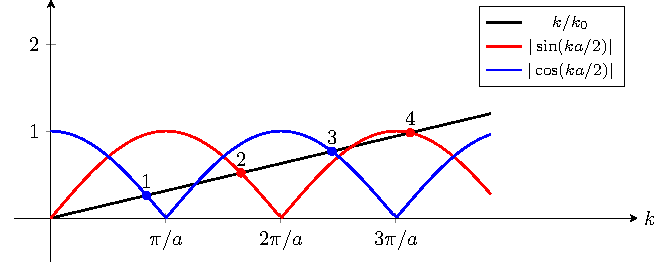
\includegraphics{images/chap2-puits_fini_solutions.pdf}
  \caption{Résolution graphique d'une équation de Schrödinger. Partant de l'équation, une séparation a été faite en 3 zones, donnant des états d'énergie possibles au sein de la barrière (états \textbf{liés}) caractérisés par le nombre $k$. Les énergies des états liés sont ceux dont le $k$ donne un point d'intersection sur la figure.}
\end{figure}

De ce graphe nous tirons l'information suivante.
Dépendant de la pente $1/k_0$, un certain nombre d'états liés peuvent exister. Particulièrement, lorsque $1/k_0  \geq A/(\pi a)$ (autrement dit $k_0 \leq \pi a$), alors la particule n'a qu'un seul état lié au potentiel. De manière générale, si $(n-1)\pi/a \leq k_0 \leq n\pi/a$, la particule aura $n$ états liés.



\subsection{Marche de potentiel}
Une marche de potentiel est similaire au puits fini mais avec un potentiel positif. Ce potentiel s'oppose donc à l'énergie de la particule et c'est pour cette raison qu'on parle souvent de "barrière de potentiel".

\begin{figure}[h]
  \centering
  \scalebox{1.2}{%\documentclass{standalone}
%\usepackage{tikz, xcolor, amsmath}

%\begin{document}
\begin{tikzpicture}
    \draw[thick, ->] (-1,0) --+ (6,0) ;
    \draw[thick, ->] (0,-0.5) --+ (0,3.5) ;
    \draw[thick, red] (0.1, 0.1) -- (0.1, 2) -- (3, 2) -- (3, 0.1) ;
    \draw[thick, red, dashed] (-1, 0.1) -- (0.1, 0.1) ;
    \draw[thick, red, dashed] (3, 0.1) -- (4, 0.1) ;
    \draw (3, 0.07) -- (3, -0.2) node[below] {$L$} ;
    \node at (-0.5, 2) {$V_0$} ;
    \node at (7, 1.5) {$\boxed{V(x) = \begin{cases}
    0 &x\leq 0 \\
    V_0 & 0 < x < L \\
    0 &x\geq L \\
    \end{cases}}$
    } ;
    
\end{tikzpicture}
%\end{document}}
  \caption{Illustration d'un puits de potentiel fini de largeur $a$ et de profondeur $V_0$.}
  \label{fig:chap2-marche_potentiel}
\end{figure}

\subsubsection{Comparaison avec la mécanique classique}
\begin{wrapfigure}{r}{0.6\textwidth}
  \centering
  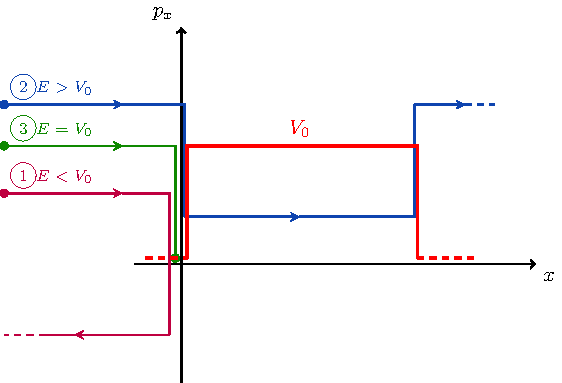
\includegraphics[width=.9\linewidth]{marche_potentiel_classique.pdf}
  \caption{Impact sur la trajectoire dans l'espace des phases (axes : position et impulsion, vitesse constante = ligne droite) d'une particule qui passe à travers une marche de potentiel.}
  \label{fig:ch2-marche_potentiel_classique}
\end{wrapfigure}

Etudier ce cas est très intéressant car une marche de potentiel en physique quantique donne un résultat extrêmement différent de la physique classique. En effet, en physique classique, une particule arrivant avec une énergie inférieure à $V_0$ rebondira. Avec une énergie supérieure à $V_0$, elle sera ralentie dans le potentiel (potentiel constant veut dire "force nulle" donc la particule a quoi qu'il arrive une vitesse constante) et repart avec sa vitesse initiale. Avec une énergie $E= V_0$, elle s'arrête.  Ces discussions sont reprises sur la figure ci-contre. \\

Pour ce qui est de la physique quantique, il faut passer par une résolution de l'équation de Schrödinger. Comme pour le puits de potentiel, écrivons l'équation dans les différentes zones et écrivons les conditions de raccordement. Notons que la forme des solutions obtenues diffère selon si $E>$ ou $< V_0$.
\subsubsection{Résolution lorsque $E > V_0$}
Nous pouvons poser le nombre 
$$k_2 = \sqrt{\dfrac{2m(E-V_0)}{\hbar}}$$
de sorte à ce qu'il soit réel, et séparer en zones comme fait pour le puit de potentiel fini.
\begin{equation}
  -\dfrac{\hbar^2}{2m} \partial_x ^2 \varphi = (E-V(x)) \varphi 
  \quad \Rightarrow \quad \ \left\{ 
    \begin{array}{lll}
      \text{Zone I} & V = 0 & -\dfrac{\hbar^2}{2m} \partial_x ^2 \varphi = E \varphi \\
      \text{Zone II} & V = V_0 & -\dfrac{\hbar^2}{2m} \partial_x ^2 \varphi = (E-V_0) \varphi \\
      \text{Zone III} & V = 0 & -\dfrac{\hbar^2}{2m} \partial_x ^2 \varphi = E \varphi \\
    \end{array}
    \right. 
  \end{equation}
  Ces équations sont simples à résoudre, et donnent :
  \begin{align}
    \varphi_{\mathrm{I}}(x) &= A_1 e^{k_1 x} + A' _1 e^{-k_1 x} \\
    \varphi_{\mathrm{II}}(x) &= A_2 e^{ik_2 x} + A' _2 e^{-ik_2 x} \\
    \varphi_{\mathrm{III}}(x) &= A_3 e^{k_1 x} + A' _3 e^{-k_1 x} 
  \end{align}
  où
  $$
    k_1 = \sqrt{-\dfrac{2mE}{\hbar}} \quad \in \mathbb{C} 
  $$
Les considérations physiques et les conditions de raccord impliquent encore des relations entre les coefficients. Notamment :

\begin{align}
  A_1 &= \left[\cos(k_2 L) - i \; \dfrac{k_1 ^2 + k_2 ^2}{2k_1k_2} \; \sin(k_2L) \right] e^{ik_1L}A_3 \\
  A_1 ' &= i \; \dfrac{k_2 ^2 - k_1 ^2}{2k_1 k_2}\; \sin(k_2L) \; e^{ik_1L} A_3
\end{align}

Une manière d'interpréter la physique du système est d'observer les ainsi nommés \textbf{coefficients de transmission et de réflexion}. Comme leur nom l'indique, ces coefficients quantifient la probabilité que la particule traverse la barrière et la probabilité qu'elle soit réfléchie en la rencontrant. Ainsi, ces coefficients seront toujours exprimés comme un rapport où le dénominateur est $A_1$ : le coefficient de la partie de la fonction d'onde qui symbolise une particule se dirigant vers les $x>0$ avec un nombre d'onde $k_1$, soit l'état initial de la particule.\\

De là, la réflexion de la particule sera lue dans le coefficient $A_1'$, qui correspond à une fonction d'onde dans la zone 1 de nombre d'onde $k_1$ se propageant vers la gauche.

$$ R = \left|\dfrac{A_1'}{A_1}\right|^2$$

La transmission sera caractérisée par le coefficient $A_3$, qui multiplie une fonction d'onde dans la zone 3 se déplaçant avec un nombre d'onde $k_1$ vers la droite.

$$ T = \left|\dfrac{A_3}{A_1}\right|^2$$

Les calculs dans ce cas précis montrent que :
\begin{align}
  R &= \dfrac{(k_1 ^2 - k_2 ^ 2) ^2 \sin^2(k_2 L)}{4k_1 ^2 k_2 ^2 + (k_1 ^2 - k_2 ^ 2) ^2\sin(k_2L)} \\
  T &= \dfrac{4k_1 ^2 k_2 ^2}{4k_1 ^2 k_2 ^2 + (k_1 ^2 - k_2 ^ 2) ^2\sin(k_2L)} 
\end{align}
Chose chouette : 
$$ R + T = 1 \; .$$
Compte tenu des définitons des $k_i$, le coefficient de transmission peut se réécrire en fonction de $E$ sous la forme suivante :
\begin{equation}
  T = \dfrac{4E (E-V_0)}{4E(E-V_0) + V_0 ^2 \sin ^ 2\left[\sqrt{2m(E-V_0)} L/\hbar\right]}
\end{equation}
On voit que le coefficient de transmission est périodique en $E$ et que sa valeur maximale est 1, lorsque le sinus s'annule. Ceci est le phénomène de \textbf{résonnance} et arrive lorsque $k_2L = n\pi$, $n\in \mathbb{Z}$.

\begin{figure}[h]
  \centering
  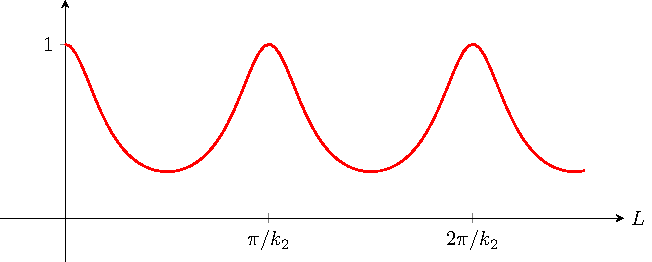
\includegraphics{marche_potentiel_transmission.pdf}
  \caption{Variation du coefficient de transmission de la barrière de potentiel en fonction de sa largeur. Résonnances aux multiples de $\pi/k_2$.}
\end{figure}

\subsubsection{Résolution lorsque $E < V_0$}
Une résolution similaire, voire même identique, s'obtient en posant $$k_2 \longrightarrow -i\rho_2 \qquad \rho_2 = \sqrt{2m(V_0-E)/\hbar ^2} \; \in \mathbb{R} $$ aux résultats déjà obtenus. Ainsi :
\begin{align}
  T = \left|\dfrac{A_3}{A_1}\right|^2 &= \dfrac{-4k_1 ^2 \rho_2 ^2}{-4k_1 ^2 \rho_2 ^2 + (k_1 ^2 + \rho_2 ^ 2) ^2\sin(-i\rho_2 L)} \\
  &= \dfrac{4E (V_0-E)}{4E(V_0-E) + V_0 ^2 \sinh ^ 2(\rho_2 L)}
\end{align}
Observons ce qui se passe lorsque la barrière est très imposante par rapport à l'énergie de la particule : $\rho_2L \gg 1$. Le sinus hyperbolique peut subir une approximation et la fraction peut se simplifier largement.
\begin{align}
\sinh(x) = \dfrac{e^{x} - e^{-x}}{2} &\Rightarrow \sinh^2(x)_{|_{x\gg 1}} \sim e^{2x}/4 \\
&\Rightarrow T \approx \dfrac{16(V_0-E)}{V_0 ^2} \; e^{-2\rho_2 L}
\end{align}
Nous voyons que lorsque la barrière est imposante (large et à haut potentiel), la particule a tout de même une probabilité non-nulle de la franchir. Ceci est propre à la mécanique quantique et ne serait jamais arrivé en mécanique classique. Ce phénomène porte le nom d'\textbf{Effet Tunnel} et possède comme application notable le microscope à effet tunnel.

\newpage
\section{Approximation semi-classique (WKB)}
Toujours dans le cadre de l'étude de l'équation de Schrödinger, nous allons dans cette section étudier une solution \textbf{approximative} de cette équation, valable dans la limite $\hbar \longrightarrow0$. Cette approximation est nommée en l'honneur de Léon Brillouin, Hendrik Anthony Kramers et Gregor Wentzel. L'idée est la suivante : en poussant $\hbar$ vers zéro, nous devrions retrouver des résultats de la mécanique classique. Abordons donc cela en écrivant premièrement l'équation de Schrödinger. Ensuite, inteprétons la solution obtenue.
\subsection{Résolution de l'équation de Schrödinger}

\begin{equation}\label{eq:ch2-WKB-schrod}
  -\dfrac{\hbar^2}{2m} \partial_x ^2 \phi + V(x)\psi = E\psi
\end{equation}

Posons $\psi(x) = A(x) e^{i\; S(x)/\hbar}$. Pour remplacer dans \ref{eq:ch2-WKB-schrod}, calculons d'abord les dérivées de $\psi$ en fonction de $A$ et $S$ et écrivons ce que donne l'équation de Schrödinger.
\begin{align}
  \psi' &= \left[ A' + \dfrac{i}{\hbar} S' A\right]e^{i\; S/\hbar} \\
  \psi'' &= \left[A'' + \dfrac{i}{\hbar} (S''\; A + S'\; A') - \dfrac{1}{\hbar ^2} S^{\prime 2} A + \dfrac{i}{\hbar} S' \; A'\right] e ^{i\; S/\hbar} \\
  \Rightarrow -&\dfrac{\hbar ^2 }{2m} \left[A'' + \dfrac{i}{\hbar} (S''\; A + S'\; A') - \dfrac{1}{\hbar ^2} S^{\prime 2} A + \dfrac{i}{\hbar} S' \; A'\right] e ^{i\; S/\hbar} + VA e ^{i\; S/\hbar} = EA e ^{i\; S/\hbar} \label{eq:ch2-WKB-SchrodAS}
\end{align}
En séparant les parties réelle et imaginaire de l'équation \ref{eq:ch2-WKB-SchrodAS}, on obtient le système suivant. Ce système est l'équivalent de \ref{eq:ch2-WKB-schrod}.
\begin{align}
      2S' \; A' + A \; S'' &= 0 \label{eq:ch2-WKB-SchrodAS-Im} \\
      \dfrac{S^{\prime 2}}{2m} - \dfrac{\hbar ^2}{2m} \dfrac{A''}{A} + V &= E \label{eq:ch2-WKB-SchrodAS-Re} 
\end{align}
L'équation \ref{eq:ch2-WKB-SchrodAS-Im} a une solution exacte. Elle est donnée par 
\begin{equation}
  A(x) = \dfrac{A_0}{\sqrt{S'(x)}}
\end{equation}
L'équation \ref{eq:ch2-WKB-SchrodAS-Re} peut être modifiée par notre approximation $\hbar \longrightarrow 0$, car alors $\hbar ^2/2m \longrightarrow 0$. L'équation obtenue est \textbf{l'équation de Hamilton-Jacobi}\footnote{Retenez bien ce nom car il m'a valu 4 points sur 20 à l'examen de Mécanal}.
\begin{equation}
  \dfrac{S^{\prime 2}}{2m} + V(x) = E
\end{equation}
En posant $p(x) = \sqrt{2m[E - V(x)]}$, on obtient aisemment
\begin{equation}
  S(x) = \pm \int ^x \d x' p(x')
\end{equation}
Et la fonction d'onde prend alors la forme suivante :
\begin{equation} \label{eq:ch2-WKB-solution}
  \psi(x) = \pm \dfrac{A_0}{\sqrt{p(x)}} e^{\pm i \; \int ^x \d x' p(x')/\hbar}
\end{equation}

\subsection{Interprétation de la solution}

\subsubsection{La vitesse de groupe du paquet d'onde est la vitesse classique}
L'impulsion de la particule est donnée par la fonction $p$. Calculons le nombre d'onde par la relation de De Broglie pour le nombre d'onde. Ce résultat sera important pour obtenir la vitesse de groupe. Il est important de saisir ici que le nombre d'onde dépend de la position.
$$k(x) = \dfrac{p(x)}{\hbar}$$
La vitesse de groupe $v_g$ est donnée par $\d\omega/\d k$. Alors on fait les physiciens et on renverse la fraction pour dériver $k$ par rapport à $\omega$ qu'on exprime comme $E/\hbar$. Alors :
$$\dfrac{1}{v_g} = \dfrac{\d k}{\d \omega} = \dfrac{\d (p/\hbar)}{E/\hbar} = \dfrac{\d p }{\d E} = \dfrac{m}{p(x)}=  \dfrac{1}{v_{\text{classique}}}$$
Ainsi, nous voyons que l'approximation semi-classique mène à une solution de l'équation de Schrödinger qui, une fois utilisée pour construire des paquets d'onde pour constituer une particule, donne une vitesse de groupe égale à la vitesse classique de la particule.

\subsubsection{Région classiquement permise et région classiquement interdite}
La région classiquement permise est définie par l'ensemble des $x$ où $V(x) < E$. Dans cette région, on peut voir par la forme \ref{eq:ch2-WKB-solution} de la fonction d'onde que la probabilité de présence de la particule est inversement proportionnelle à l'impulsion. Ceci est le cas car pour $E>V$, $p\in \mathbb{R}$ donc l'exponentielle dans \ref{eq:ch2-WKB-solution} reste imaginaire donc son module reste 1. On voit alors que la probabilité de présence diminue quand l'impulsion de la particule augmente, ce qui rejoint notre intuition\footnote{De toute façon quand ça parle de mécanique classique, tout rejoint un peu notre intuition.}.
\begin{center}
  Région classiquement permise : $E>V(x) \quad \Rightarrow \quad |\psi|^2 \propto \dfrac{1}{p}$
\end{center}

Dans la zone interdite, $E<V$ et l'impulsion devient alors imaginaire. L'exponentielle devient réelle et la probabilité de présence devient proportionnelle à une exponentielle négative, mais pas nulle ! On retrouve ici l'effet tunnel déjà discuté, mais ici pour un potentiel quelconque qui est supérieur à l'énergie. Attention : on ne retrouve que l'exponentielle négative car les considérations physiques (fonction d'onde bornée) imposent un coefficient nul à l'exponentielle croissante (pour éviter qu'elle explose à l'infini).
\begin{center}
  Région classiquement interdite : $E<V(x) \quad \Rightarrow \quad |\psi|^2 \propto e^{-\int ^x p(x') \d x'}$
\end{center}

Les figures ci-dessous reprennent un cas de potentiel et l'allure de la fonction d'onde correspondante. On voit aux lignes verticales pointillées, qui correspondent aux frontières entre les régions permise et interdite, que la probabilité devient exponentiellement décroissante mais non nulle (effet tunnel).
\begin{figure}[h]
  \centering
  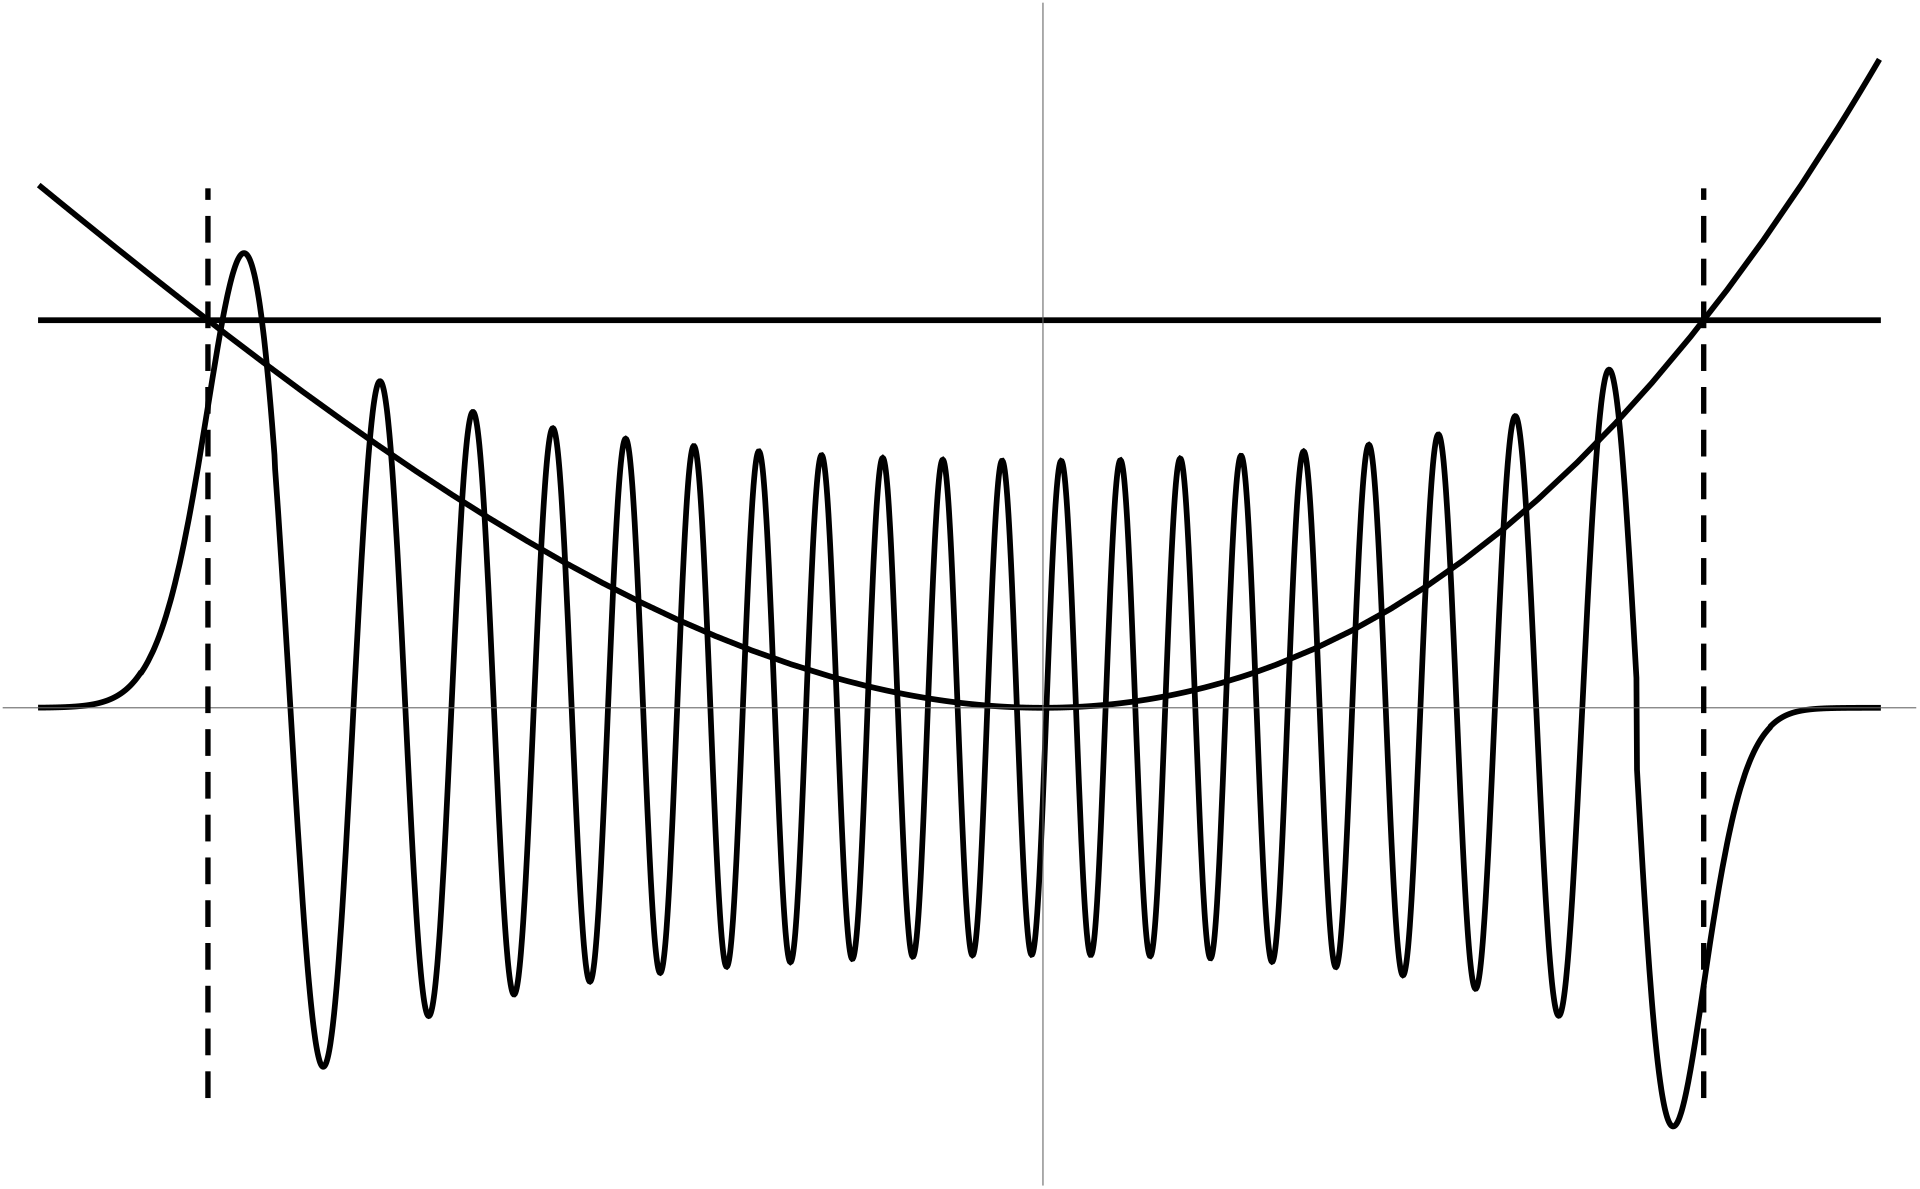
\includegraphics[width=.4\linewidth]{WKB_approximation_example.svg.png} \\ 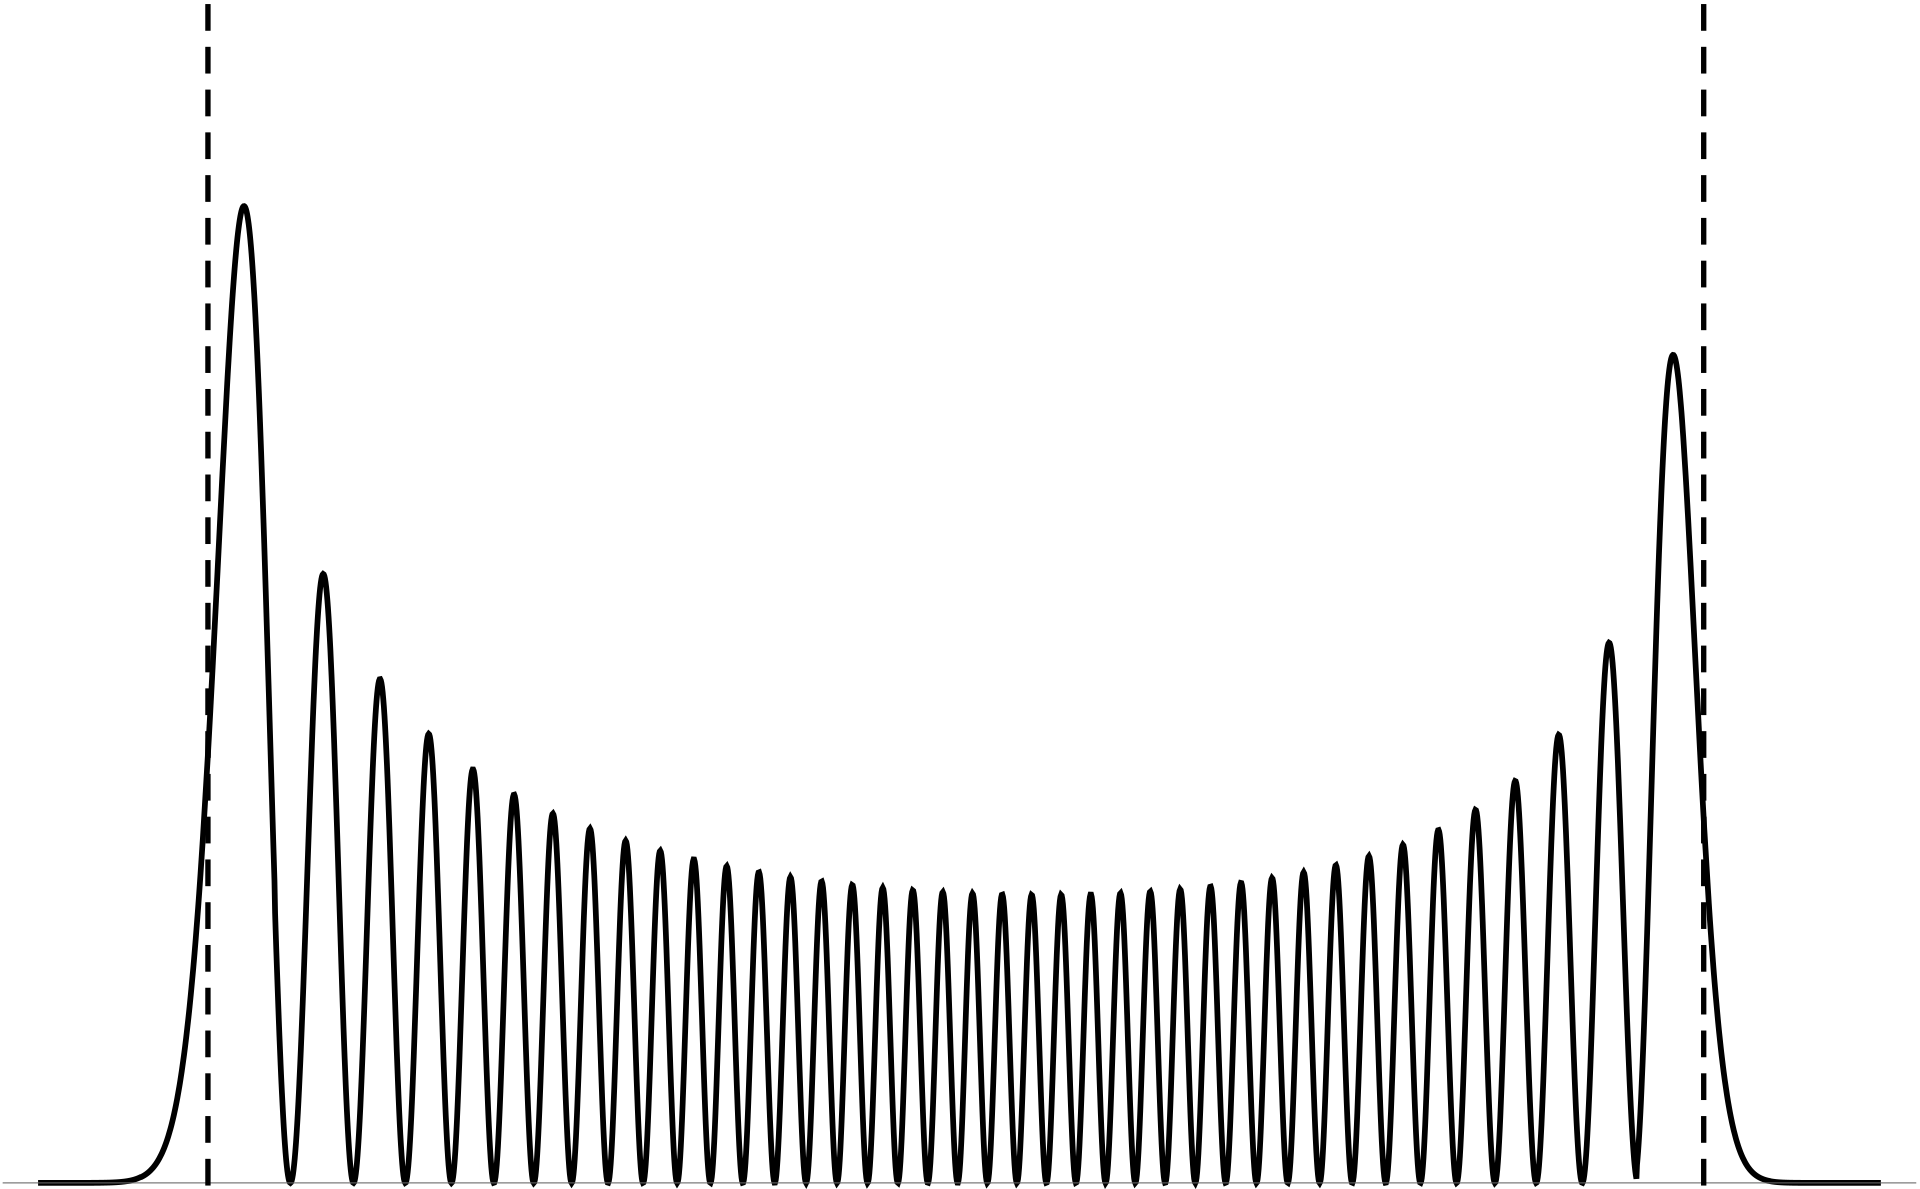
\includegraphics[width=.4\linewidth]{WKB_approximation_example_2.svg.png}
  \caption{Graphe d'une fonction d'onde d'une particule et de sa densité de probabilité de présence sous l'approximation WKB.}
\end{figure}

\subsubsection{Etats liés}
Si nous sommes dans le cas d'une solution qui décroit exponentiellement à grande distance, en notant $b$ et $a$ les points de rebroussement de la trajectoire classique, les états liés, dans la région permise donc, sont décrits par les fonctions suivantes, selon si on est proche de la frontière gauche avec la région interdite ou la frontière droite :
\begin{equation}
  \begin{array}{llr}
    \psi(x) &= \dfrac{1}{\sqrt{k(x)}} \; \cos\left[\int_b ^x k(x')\; \d x' \quad - \pi/4\right] & x>b \\   
    \psi(x) &= \dfrac{1}{\sqrt{k(x)}} \; \cos\left[\int_x ^a k(x')\; \d x' \quad + \pi/4\right] & x<a    
  \end{array}
\end{equation}
Une condition de quantification est que la somme des phases des cosinus soit égale à un multiple de $\pi/2$ \rouge{confirmation needed, source wikipedia}. En sommant sur le domaine d'intégration, on obtient l'intégrale du nombre d'onde entre les deux points de rebroussement (les points de frontière).
\begin{center}
  Condition de quantification semi-classique : $\dfrac{1}{\hbar} \int_b ^a \dx \sqrt{2m(E-V(x))} \quad = \left(n+\dfrac{1}{2}\right) \pi$
\end{center}

\subsection{Application de l'approximation WKB en physique nucléaire}
Illustrons les résultats obtenus concernant l'approximation WKB d'un exemple d'application qui est celui de la désintégration-$\alpha$,
mettant en avant la loi de Geiger-Nuttal. \\
%Explication sur la raison pour laquelle cette approximation est d'application 

Avant de rentrer dans les détails, rappelons ce que sont un temps de demi-vie $t_{1/2}$ et la désintégration alpha : 
\begin{itemize}[label = \textbullet]
  \item \textbf{Désintégration $\alpha$} $\equiv$ (wikipédia {\color{red}{à vérifier}}) forme de désintégration radioactive où un noyau atomique éjecte une particule $\alpha$
  ( $= He^{++}$) et se transforme en un noyau plus léger ; 
  \item \textbf{Demi-vie $t_{1/2}$} d'un isotope radioactif $\equiv$ (wikipédia) c'est le temps au bout duquel la moitié des noyaux de cet isotope initiaux se sont désintégrés. \\
  Notons qu'il est important de reconnaître la différence entre cette définition et celle d'un temps moyen : 2 fois le temps de demi-vie $\ne$ la vie complète!!  
\end{itemize}

Considérons un noyau de rayon $R$ qui contient des particules $\alpha$ possédant une énergie $E$. 
Les particules $\alpha$ sont confinées dans le noyau, autrement dit leur énergie est plus faible que le potentiel qui les retient.
Or, nous avons déjà vu qu'une particule pouvait traverser une zone classiquement interdite par effet tunnel, et se propage comme une onde "evanescente" (qui décroît exponentiellement) dans cette zone. \\
C'est en fait ce qu'il va se passer ici pour les particules $\alpha$, initialement confinées dans le noyau. 
A la sortie du noyau, le potentiel ressenti par les particules $\alpha$ est simplement le potentiel coulombien créé par les charges du noyau. Ainsi, pour tout $r > R$, le potentiel s'écrit comme suit :
\begin{equation}
  V(r) = \frac{z_{\alpha} z e^2}{4 \pi \epsilon_0 r} %pour un potentiel crée par une charge z, on ne devrait pas avoir juste z dans cette expression au lieu de z_alpha *z ?
\end{equation}
où $z_{\alpha}$, $z$ $\equiv$ charges du noyau
%+ graphe qui illustre le potentil vu par les particules alpha

Notons $R_{\alpha}$ la distance à partir de laquelle l'énergie $E$ de la particule devient plus grande que le potentiel coulombien ressenti $V(r)$, autrement dit, $R_{\alpha}$ est la distance au noyau à partir de laquelle la particue devient libre et peut se propager de manière semi-classique (c'est-à-dire tel que la longueur d'onde varie très peu sur une distance égale à la longueur d'onde même).








\begin{appendix}
\chapter{Calculs des coefficients des fonctions d'onde}
  \section{Puits de potentiel fini} \label{annexe-CalculCoefficients-PuitsFini}
  D'entrée, nous pouvons imposer que le coefficient $B_3$ doit s'annuler pour pas que la fonction soit bornée dans la zone III(en particulier, ne tende vers l'infini quand $x$ tend vers l'infini). Il en va de même pour la zone I où nous devons fixer $B_1 '$ à zéro. $$B_3 = B_1 '=  0 $$

Les \textit{conditions de raccord} imposent que la fonction soit \textit{continue} et que sa dérivée première le soit aussi. Nous devons donc vérifier ces conditions aux frontières des zones, endroits d'éventuelles discontinuités, et imposer la continuité par les coefficients.
\subsubsection{Conditions de raccord en $x=-a/2$}
\begin{align}
  \varphi_{\mathrm{I}}(-a/2) = \varphi_{\mathrm{II}} (-a/2) &\iff A_2 = e^{-(\rho + ik) a/2} \;  \dfrac{\rho + ik}{2ik} \; B_1 \\
  \varphi_{\mathrm{I}} '(-a/2) = \varphi_{\mathrm{II}} ' (-a/2) &\iff A_2 ' =  -e^{-(\rho  + ik)a/2} \; \dfrac{\rho - ik}{2ik} \; B_1 
\end{align}

\subsubsection{Conditions de raccord en $x=a/2$}
\begin{align}
  \varphi_{\mathrm{II}}(a/2) =  \varphi_{\mathrm{III}}(a/2)\\
  \varphi_{\mathrm{II}}'(a/2) =  \varphi_{\mathrm{III}}'(a/2)
\end{align}
\end{appendix}

\end{document}
